\documentclass[10pt,letter]{article}
\usepackage[utf8]{inputenc}
\usepackage{amsmath}
\usepackage{amsfonts}
\usepackage{amssymb}
\usepackage{graphicx}
\usepackage[margin=1in]{geometry}
\usepackage{float}


\begin{document}

\begin{titlepage}
\title{PHYS 5794 Homework 6}
\date{March 14, 2016}
\author{Thomas Edwards}
\maketitle
\end{titlepage}

\section{Problem 1}

\subsection{Problem Statement}

Write a code to solve the Laplace equation by using the relaxation method.

$$ \frac{\partial^2\phi}{\partial x^2} + \frac{\partial^2\phi}{\partial y^2} = 0 $$

with

$$ \phi(x,y=0) = x(1-x), \phi(x, y=\infty) = 0, 0 \le x \le 1$$
$$ \phi(x=0,y) = 0, \phi(x=1, y) = 0, 0 \le y \le \infty$$

(i) Construct the “energy” functional $E$ whose variation with respect to $\phi$ gives rise to the
Laplace equation that you would like to solve.

(ii) Write the discretized forms of the “energy” functional and the differential equation to solve
$(\partial E / \partial \phi_{ij} )$.

(iii) For a given lattice spacing $h$, show that the converged “energy” functional $E$ does not
depend on the values of relaxation parameter $w$. Plot $E$ vs iteration time.

(iv) What is the analytical value of $E$? Do not just quote $E$. Show all the intermediate steps
to obtain $E$ (numerical value+analytical expression) if possible.

(v) For a given relaxation parameter, use two different meshes or lattice spacings to see if $E$
converges closer to the analytical value with finer meshes.

(vi) Calculate $E$ for several meshes (lattice spacings, $h$) and obtain $E(h \rightarrow 0)$ from fitting the
data points to a polynomial function of $h$. Plot $E$ vs $h$. Use your fitting program from HW5 or
any software.

(vii) Compare your result of $E(h \rightarrow 0)$ with the analytical value of $E$.

(viii) Compare the numerical value of $\phi(x, y)$ with the analytical solution of the differential
equation.

\subsection{Method}

This problem was solved using the relaxation method described in the lecture notes. The method is as follows:

Begin by making a guess solution to your system, with imposed boundary conditions, where $\phi(x,y) = \phi_0$ wherever we are not explicitly given a boundary condition. In this case, $\phi_0$ was chosen to be 0, primarily because there is an infinite range in $y$.

Next, develop an updated solution by using a finite difference relaxation scheme. This generated a new, intermediate solution  $\phi^{n+1}(x,y)$ for the entire system. We then compare this new solution to the last solution, such that if

$$|\phi^n(x,y) -\phi^{n+1}(x,y)| < \delta$$ we consider our solution stable and return it. In this case, $\delta=10^{-13}$.

This is due to the nature of the energy function $E$, which in this case is written as 

$$E = \int_0^1\int_0^\infty \left[ \frac{1}{2}(\nabla \phi)^2 \right] dydx.$$

With small variation of $E$ with respect to $\phi$, we see that

$$\delta E = \int_0^1\int_0^\infty \left[ \frac{1}{2}(\nabla \phi \cdot \nabla\delta\phi) \right] dydx$$
which becomes
$$\delta E = \int_C \delta\phi \hat{n}\cdot \nabla \phi dl+ \int_0^1\int_0^\infty \delta\phi\left[ (\nabla \phi)^2 \right] dydx.$$

The left integral goes to zero due to the boundary conditions,
$$\frac{\delta E}{\delta\phi} =  \int_0^1\int_0^\infty \left[ (\nabla^2 \phi) \right] dydx$$
due the the non-zero boundary condition along the y-axis.

We then set this equal to zero, giving us

$$ \int_0^1\int_0^\infty \left[ (\nabla^2 \phi) \right] dydx =0.$$

This is the total energy who's derivative we must minimize.

The $E$ function is discretized by a center-differenced scheme, where
$$\phi_{ij}^{n+1} = (1-\bar{w})\phi^n_{ij} + \frac{\bar{w}}{4}\left[ \phi^n_{i+1j}+\phi^n_{i-1j}+\phi^n_{ij+1}+\phi^n_{ij-1}\right]$$
where $\bar{w} = 2w/h$ and $h$ is the given step size.

The total energy $E$ was found by numerically integrating over the entire system.

The solution was found for a number of selections of $w$ and $h$. In order to show a solution that ran in a reasonable amount of time, the $y$ domain was restricted to a maximum of $10$ instead of $\infty$, however trial runs with $100$ were also used to confirm that the solution only changed minimally.

In order to confirm that both our $\phi$ solution and our $E$ solution is correct, we must compare to the analuytic solution. This was done by separation of variables, letting
$$\phi(x,y)=X(x)Y(y)$$
and seeing that
$$\frac{X''(x)}{X(x)} = -\frac{Y''(x)}{Y(x)} = -\lambda^2$$
We see that 
$$X''(x) + \lambda^2X(x)=0,$$
and since we know that $X(0)=0$ and $X(1)=0$ from boundary, conditions, we enforce a sinusoidal solution for $X(x)$. This gives us
$$X(x) = A\sin(\lambda x) + B\cos(\lambda x).$$ Given our boundary conditions, we choose that $B=0$, and $\lambda = n \pi$, giving us $$X(x) = \sin(n \pi x) .$$

Further, we note that $$Y''(x) - \lambda^2Y(x)=0,$$ and choose a particular siolution of $$Y(y) = Ae^{-\lambda y}+Be^{\lambda y}.$$ Given that $Y(\infty) = 0$, we see that $$Y(y) = Ae^{-\lambda \infty}+Be^{\lambda \infty},$$ and thus we choose that $B=0$, giving us $$Y(y) = Ae^{-n \pi y}.$$

To find $A$ we must use a series solution, $$\phi(x,y) = \sum_{n=1}^\infty c_n e^{-n \pi x} \sin(n \pi x) $$ where $$c_n = 2\int_0^1x(1-x)\sin(n \pi x) dx$$ given our boundary condition $\phi(x,0) = x(1-x)$.

This is our analytic solution for this problem, and solving for $E$ is done in the same manner as the analytic solution, but integragtion over the entire system space.


\subsection{Verification of Program}

This program was validated by comparing to the analyitc solution, shown in the plot below.

\begin{figure}[H]
  \centering
    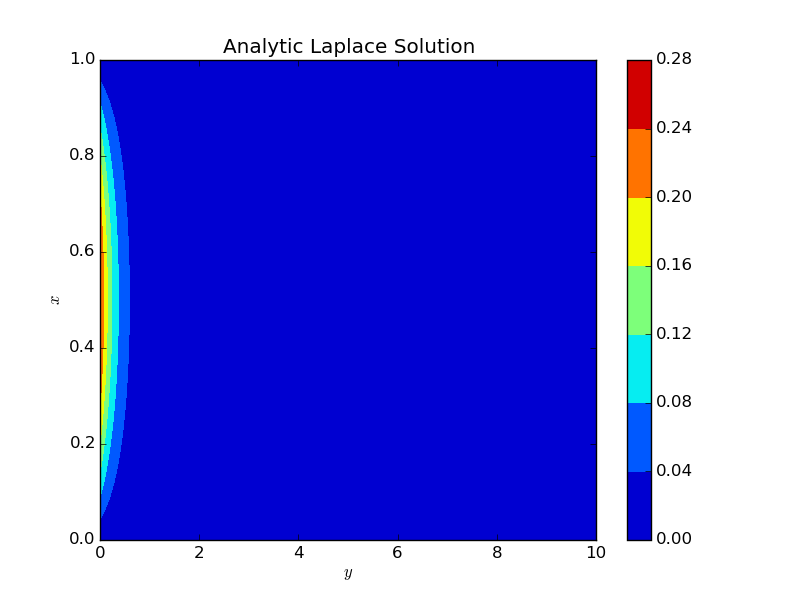
\includegraphics[width=.6\textwidth]{homework7_problem1_plot0}
\end{figure}

It will be very aparent in the later portions of this report that the numerical solution matches this solution quite well.

\subsection{Data}

The results from the algorithm are shown below.

\begin{verbatim}
------------------
Analytic E (for h=0.1):
0.0611965006177
------------------
w =  0.05
h =  0.5
Final iteration number:  185
Elapsed time:  0.101413965225
Final E:  0.0873587870738
------------------
w =  0.04
h =  0.5
Final iteration number:  231
Elapsed time:  0.0964131355286
Final E:  0.0873587870709
------------------
w =  0.03
h =  0.5
Final iteration number:  306
Elapsed time:  0.115415096283
Final E:  0.0873587870654
------------------
w =  0.02
h =  0.5
Final iteration number:  453
Elapsed time:  0.19428896904
Final E:  0.0873587870544
------------------
w =  0.01
h =  0.5
Final iteration number:  880
Elapsed time:  0.289990186691
Final E:  0.087358787022
------------------
w =  0.05
h =  0.25
Final iteration number:  320
Elapsed time:  0.488300085068
Final E:  0.0768170986201
------------------
w =  0.04
h =  0.25
Final iteration number:  398
Elapsed time:  0.644874095917
Final E:  0.076817098616
------------------
w =  0.03
h =  0.25
Final iteration number:  525
Elapsed time:  1.15135192871
Final E:  0.076817098608
------------------
w =  0.02
h =  0.25
Final iteration number:  775
Elapsed time:  1.30969882011
Final E:  0.0768170985931
------------------
w =  0.01
h =  0.25
Final iteration number:  1500
Elapsed time:  3.186658144
Final E:  0.076817098548
------------------
w =  0.05
h =  0.125
Final iteration number:  608
Elapsed time:  4.3663380146
Final E:  0.066374119856
------------------
w =  0.04
h =  0.125
Final iteration number:  754
Elapsed time:  5.02864003181
Final E:  0.066374119849
------------------
w =  0.03
h =  0.125
Final iteration number:  992
Elapsed time:  6.43330788612
Final E:  0.0663741198358
------------------
w =  0.02
h =  0.125
Final iteration number:  1460
Elapsed time:  10.2307379246
Final E:  0.0663741198108
------------------
w =  0.01
h =  0.125
Final iteration number:  2815
Elapsed time:  15.9215009212
Final E:  0.0663741197337
------------------
w =  0.05
h =  0.1
Final iteration number:  752
Elapsed time:  6.8153591156
Final E:  0.0641752611035
------------------
w =  0.04
h =  0.1
Final iteration number:  930
Elapsed time:  8.22512793541
Final E:  0.0641752610935
------------------
w =  0.03
h =  0.1
Final iteration number:  1224
Elapsed time:  10.9950239658
Final E:  0.0641752610784
------------------
w =  0.02
h =  0.1
Final iteration number:  1799
Elapsed time:  15.9751310349
Final E:  0.0641752610472
------------------
w =  0.01
h =  0.1
Final iteration number:  3466
Elapsed time:  30.4340839386
Final E:  0.0641752609538
------------------
Extrapolated E(h->0):  0.0556445906015
\end{verbatim}

The plots requested in the problem statement are shown below.

\begin{figure}[H]
  \centering
    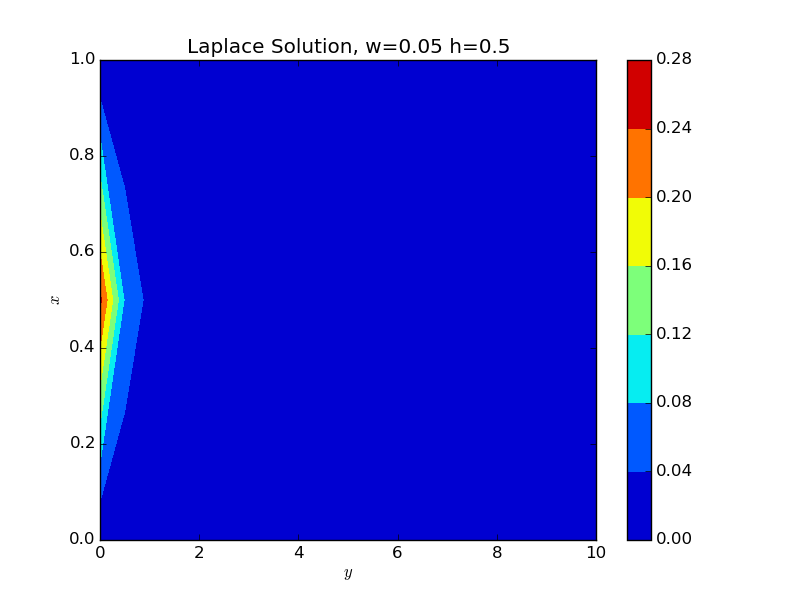
\includegraphics[width=.6\textwidth]{homework7_problem1_plot1}
\end{figure}
\begin{figure}[H]
  \centering
    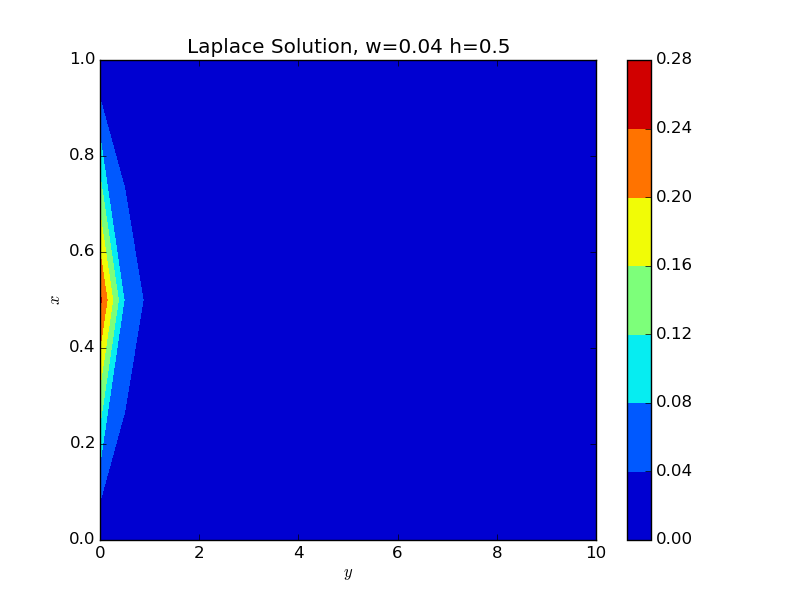
\includegraphics[width=.6\textwidth]{homework7_problem1_plot2}
\end{figure}
\begin{figure}[H]
  \centering
    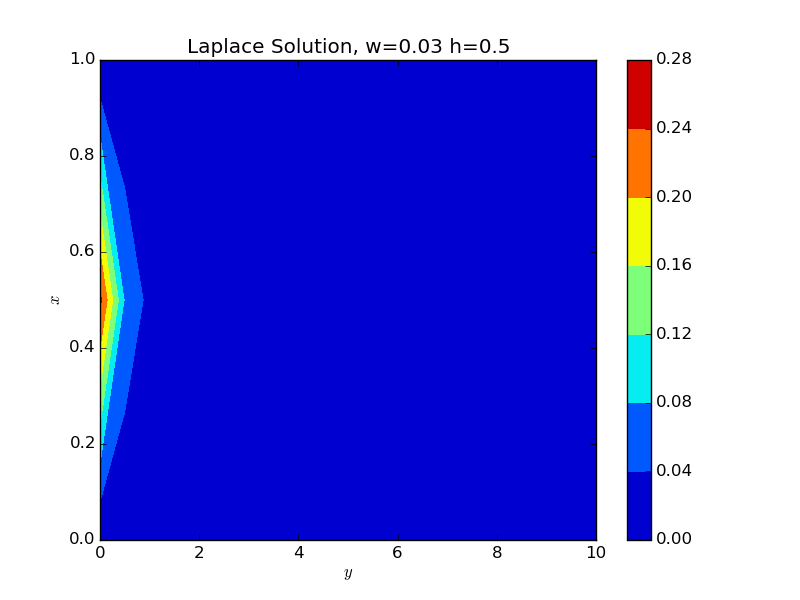
\includegraphics[width=.6\textwidth]{homework7_problem1_plot3}
\end{figure}
\begin{figure}[H]
  \centering
    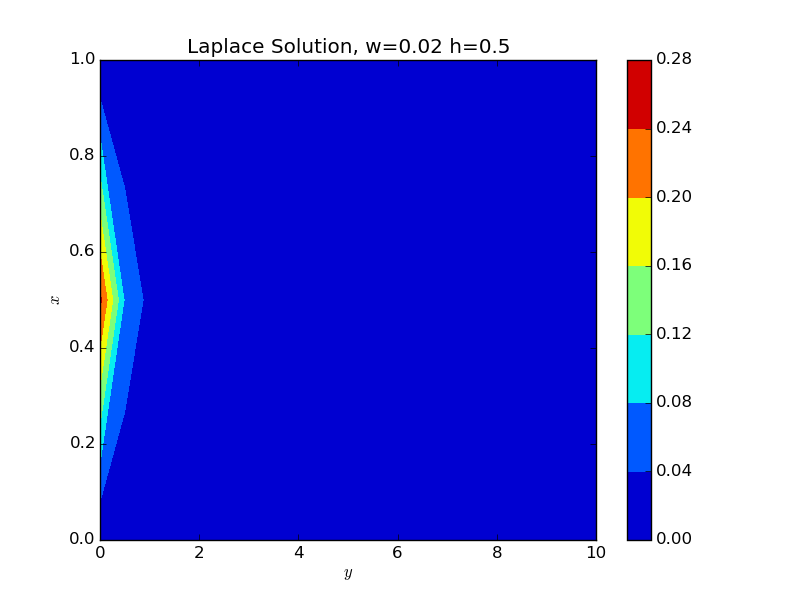
\includegraphics[width=.6\textwidth]{homework7_problem1_plot4}
\end{figure}
\begin{figure}[H]
  \centering
    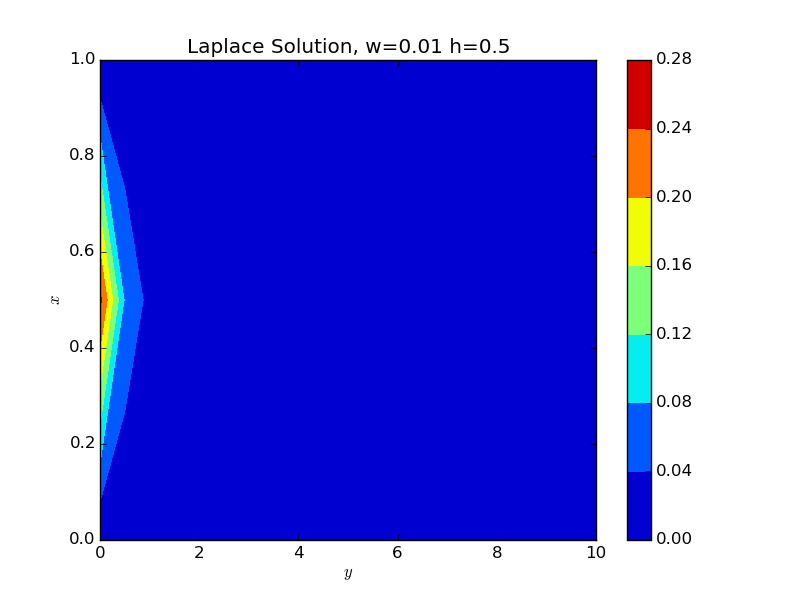
\includegraphics[width=.6\textwidth]{homework7_problem1_plot5}
\end{figure}
\begin{figure}[H]
  \centering
    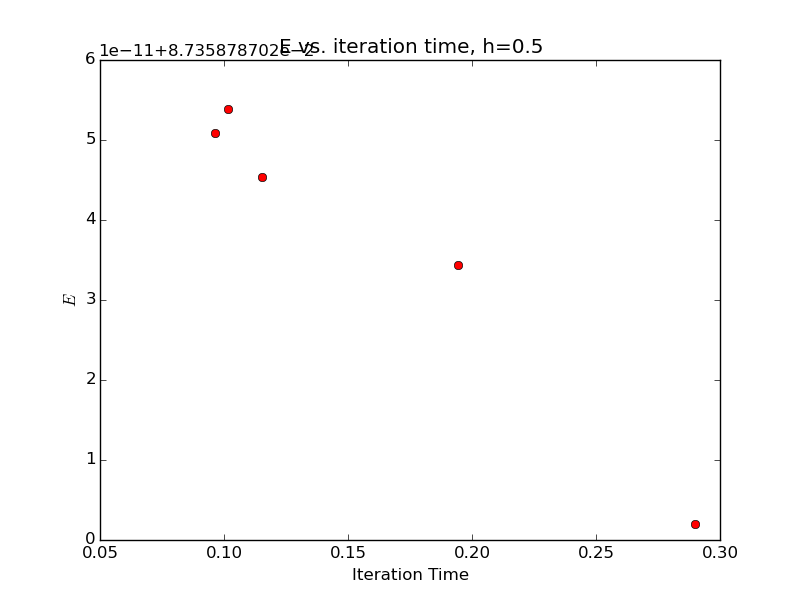
\includegraphics[width=.6\textwidth]{homework7_problem1_plot6}
\end{figure}
\begin{figure}[H]
  \centering
    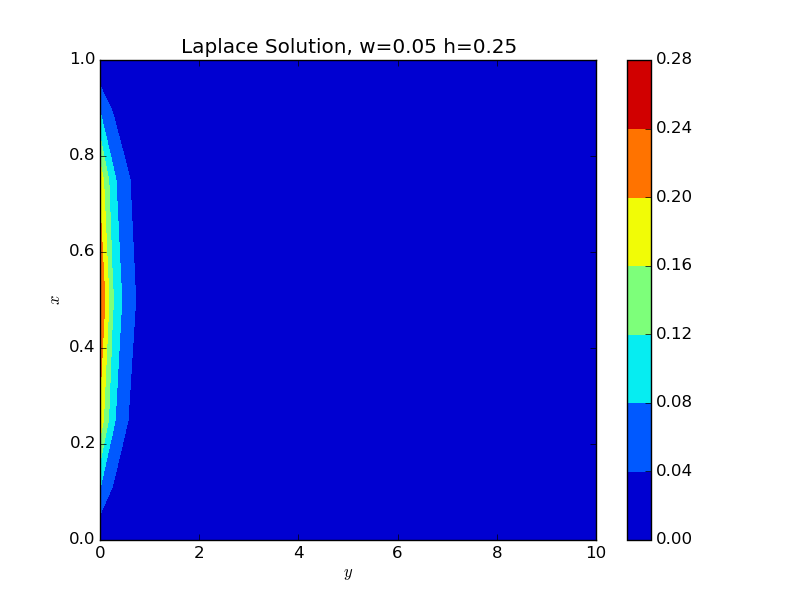
\includegraphics[width=.6\textwidth]{homework7_problem1_plot7}
\end{figure}
\begin{figure}[H]
  \centering
    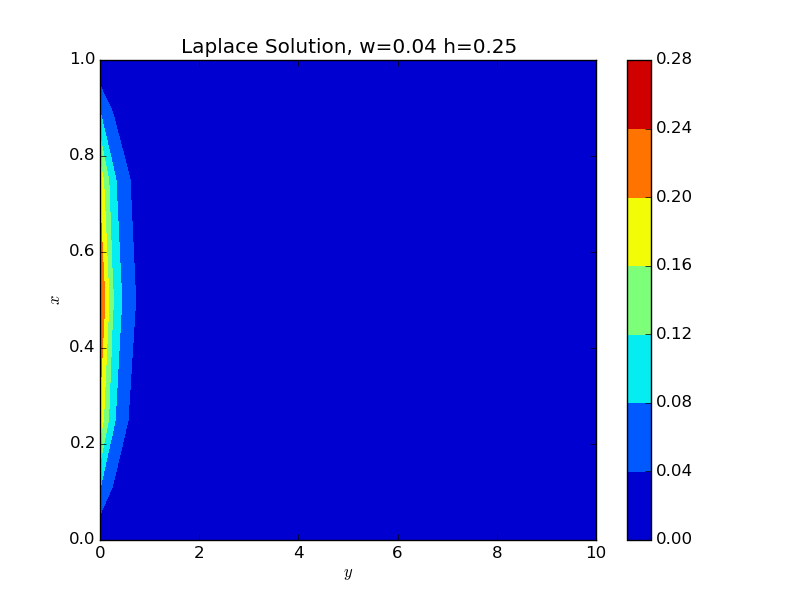
\includegraphics[width=.6\textwidth]{homework7_problem1_plot8}
\end{figure}
\begin{figure}[H]
  \centering
    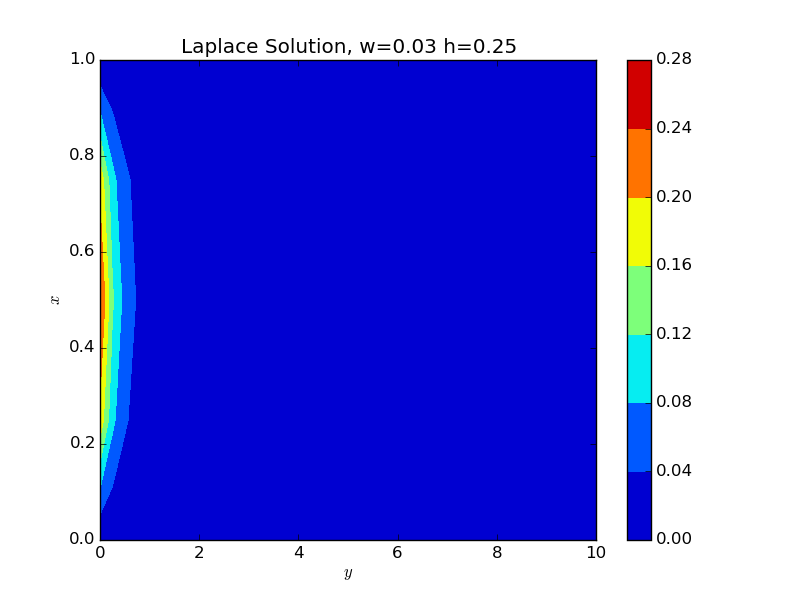
\includegraphics[width=.6\textwidth]{homework7_problem1_plot9}
\end{figure}
\begin{figure}[H]
  \centering
    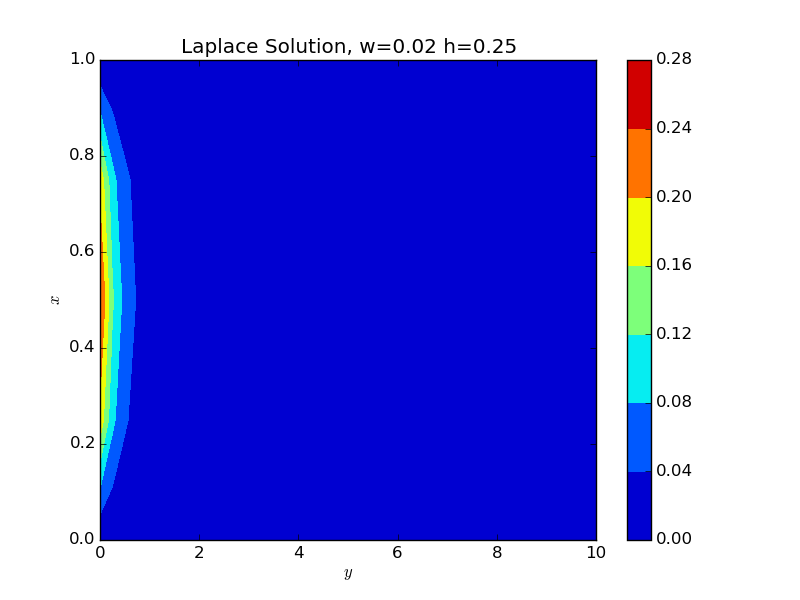
\includegraphics[width=.6\textwidth]{homework7_problem1_plot10}
\end{figure}
\begin{figure}[H]
  \centering
    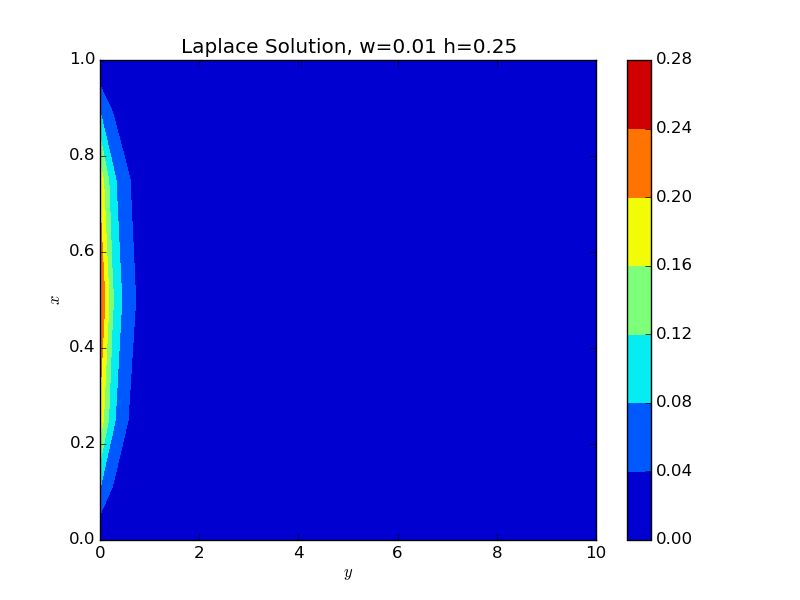
\includegraphics[width=.6\textwidth]{homework7_problem1_plot11}
\end{figure}
\begin{figure}[H]
  \centering
    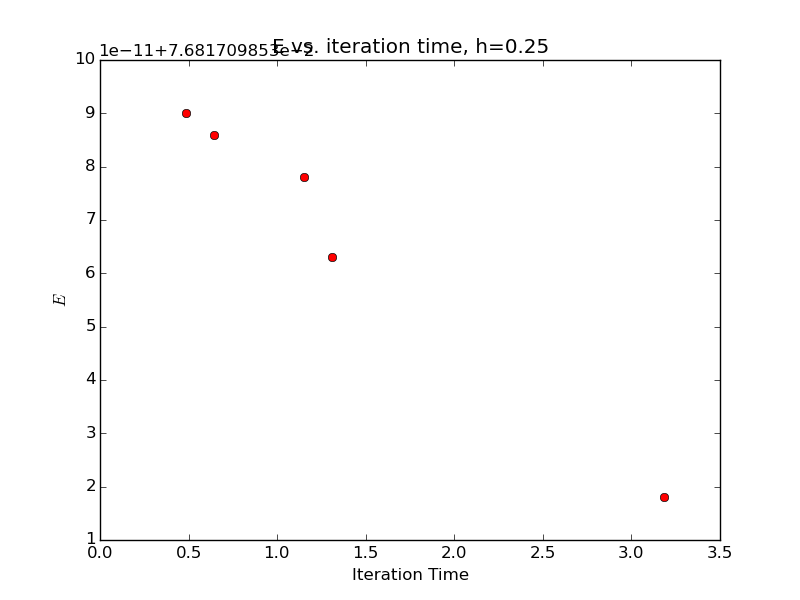
\includegraphics[width=.6\textwidth]{homework7_problem1_plot12}
\end{figure}
\begin{figure}[H]
  \centering
    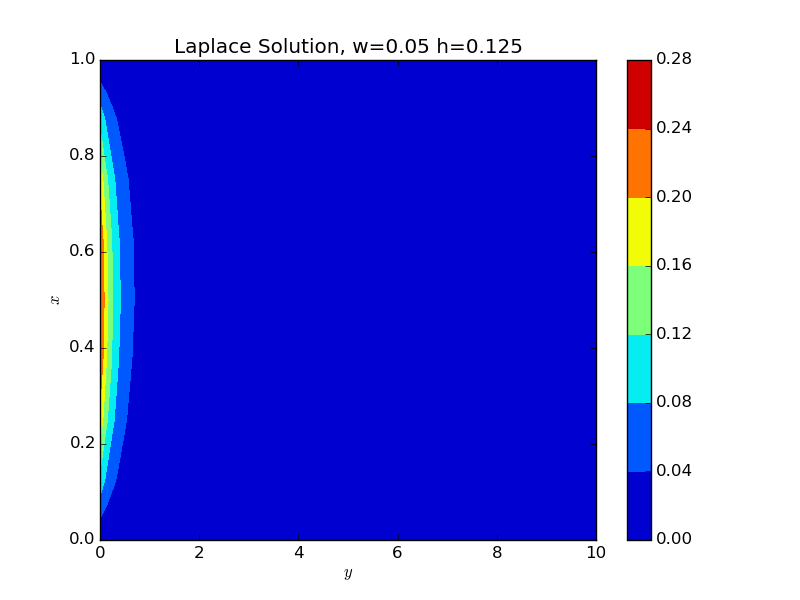
\includegraphics[width=.6\textwidth]{homework7_problem1_plot13}
\end{figure}
\begin{figure}[H]
  \centering
    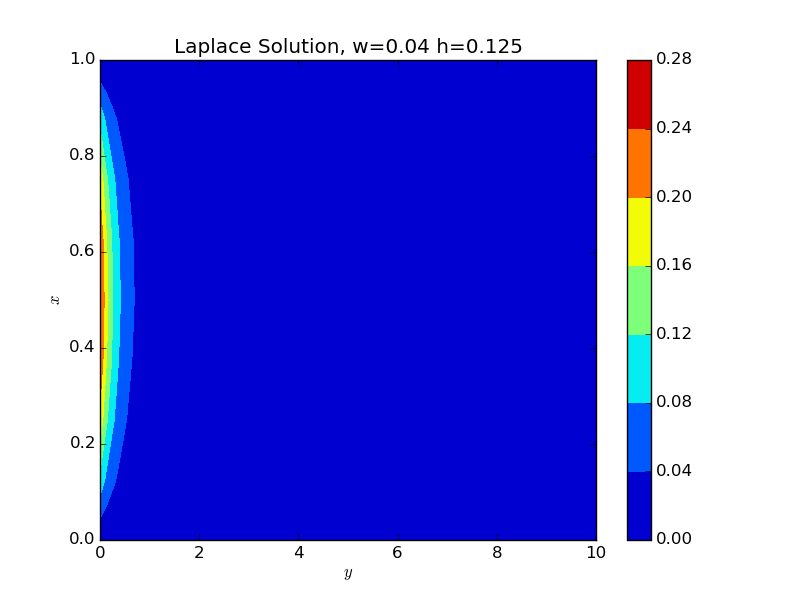
\includegraphics[width=.6\textwidth]{homework7_problem1_plot14}
\end{figure}
\begin{figure}[H]
  \centering
    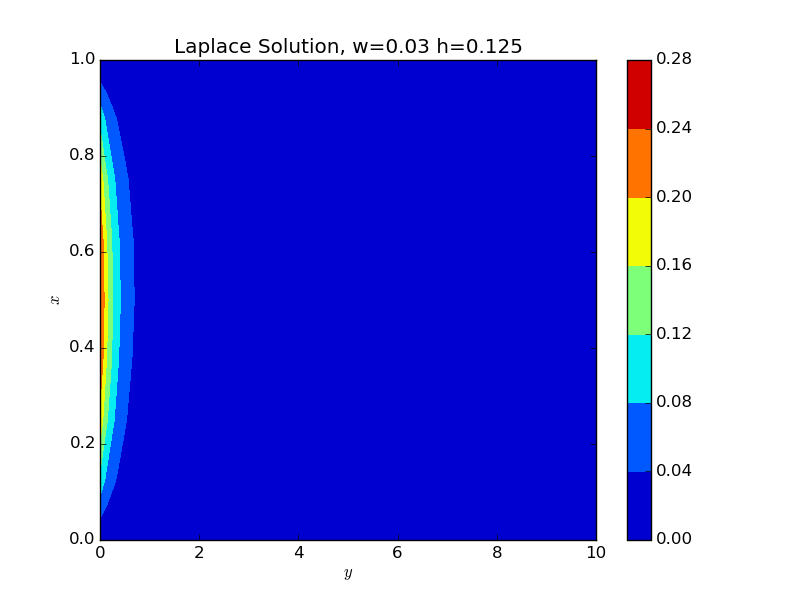
\includegraphics[width=.6\textwidth]{homework7_problem1_plot15}
\end{figure}
\begin{figure}[H]
  \centering
    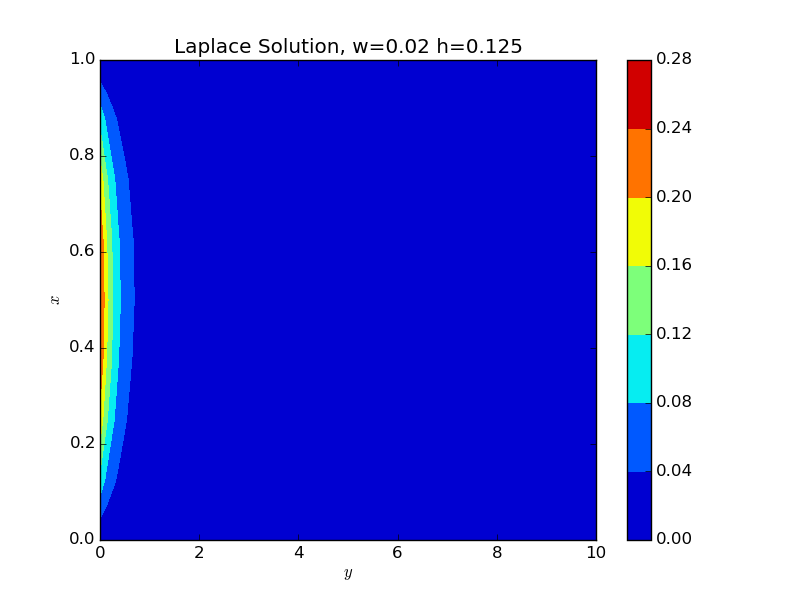
\includegraphics[width=.6\textwidth]{homework7_problem1_plot16}
\end{figure}
\begin{figure}[H]
  \centering
    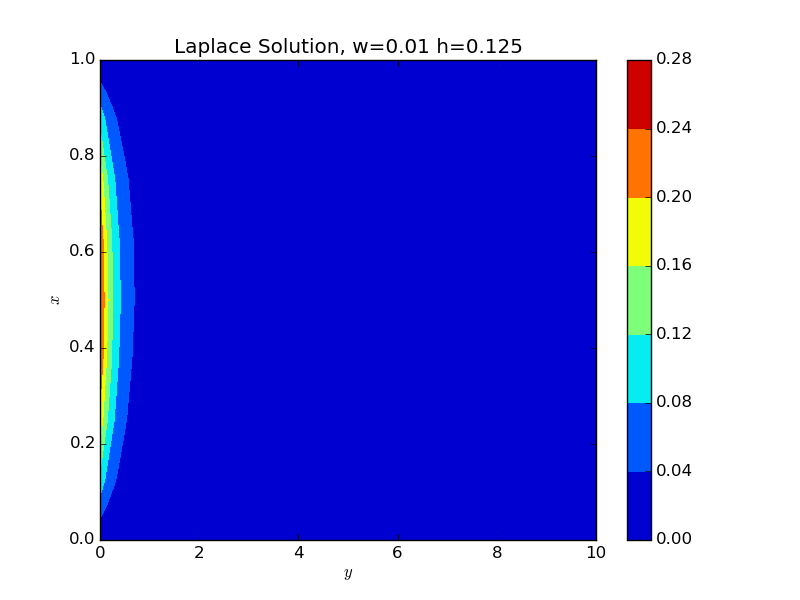
\includegraphics[width=.6\textwidth]{homework7_problem1_plot17}
\end{figure}
\begin{figure}[H]
  \centering
    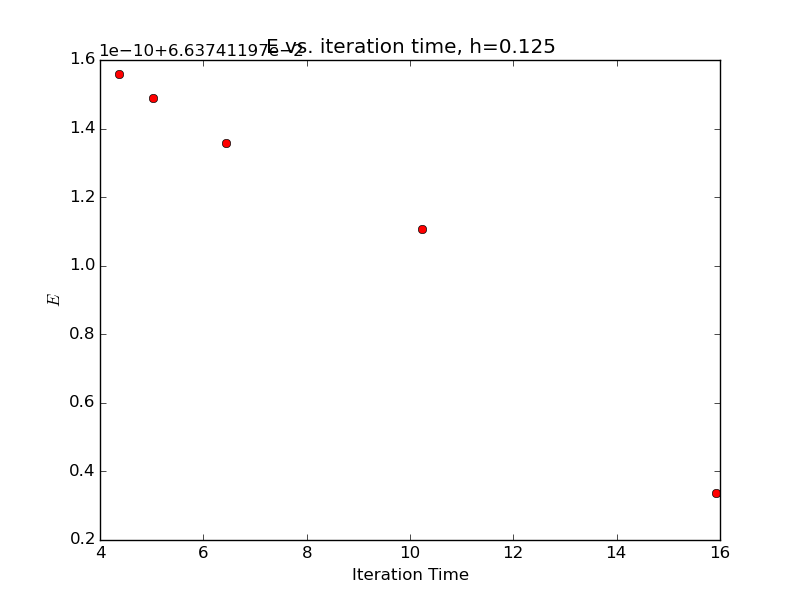
\includegraphics[width=.6\textwidth]{homework7_problem1_plot18}
\end{figure}
\begin{figure}[H]
  \centering
    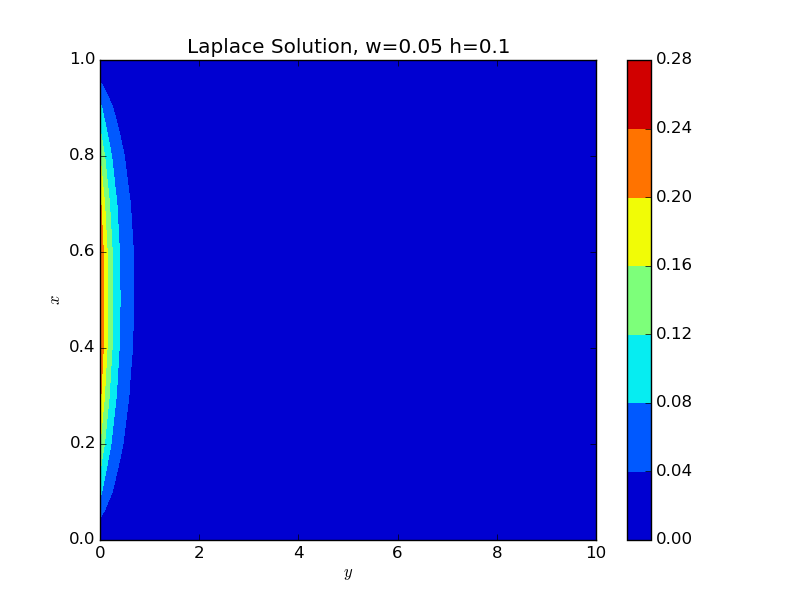
\includegraphics[width=.6\textwidth]{homework7_problem1_plot19}
\end{figure}
\begin{figure}[H]
  \centering
    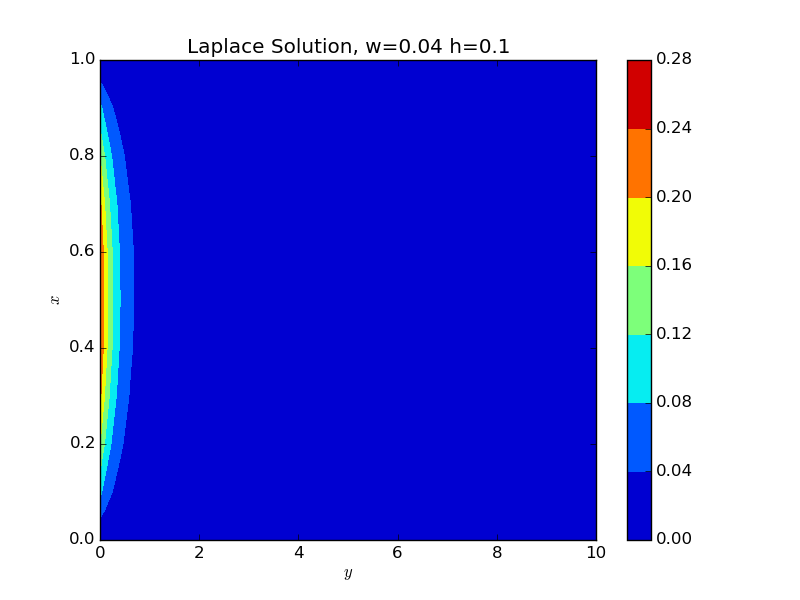
\includegraphics[width=.6\textwidth]{homework7_problem1_plot20}
\end{figure}
\begin{figure}[H]
  \centering
    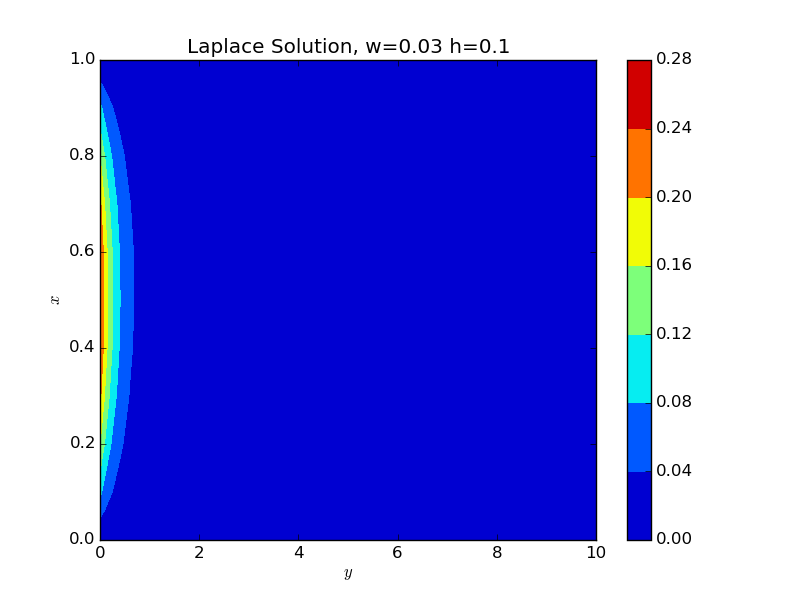
\includegraphics[width=.6\textwidth]{homework7_problem1_plot21}
\end{figure}
\begin{figure}[H]
  \centering
    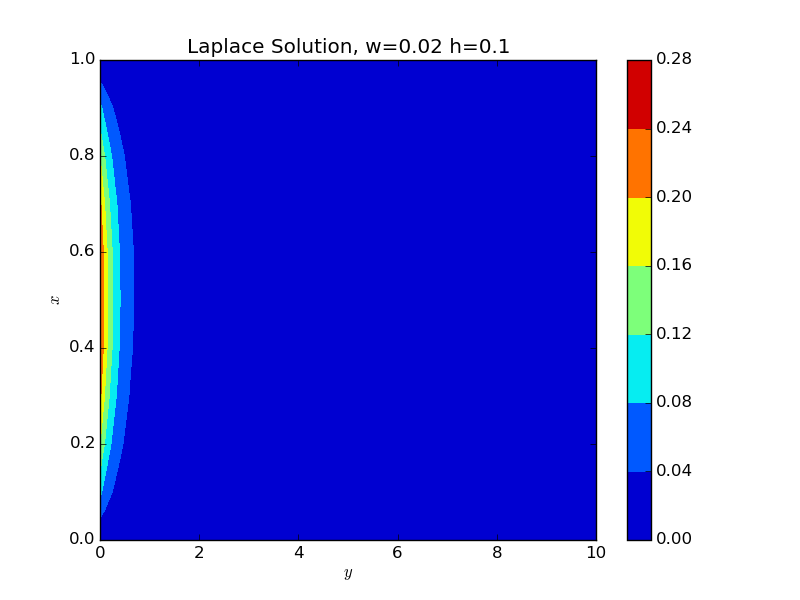
\includegraphics[width=.6\textwidth]{homework7_problem1_plot22}
\end{figure}
\begin{figure}[H]
  \centering
    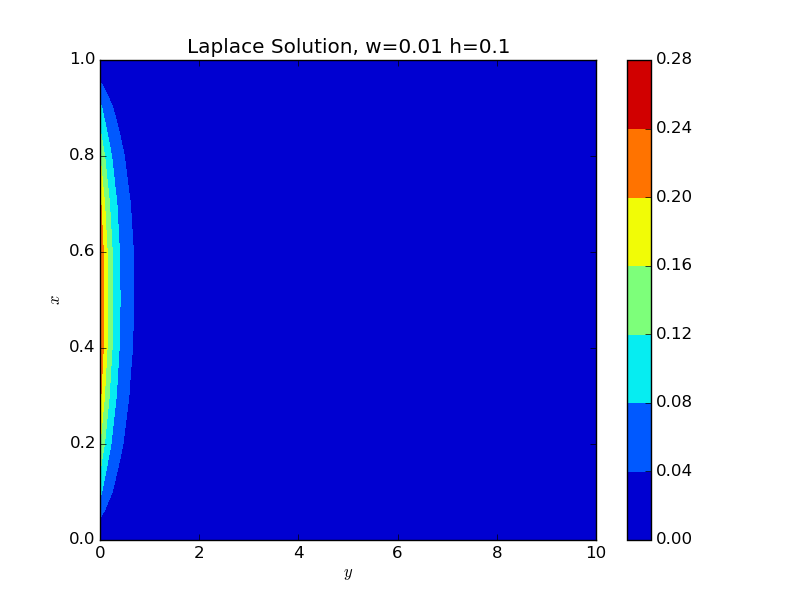
\includegraphics[width=.6\textwidth]{homework7_problem1_plot23}
\end{figure}
\begin{figure}[H]
  \centering
    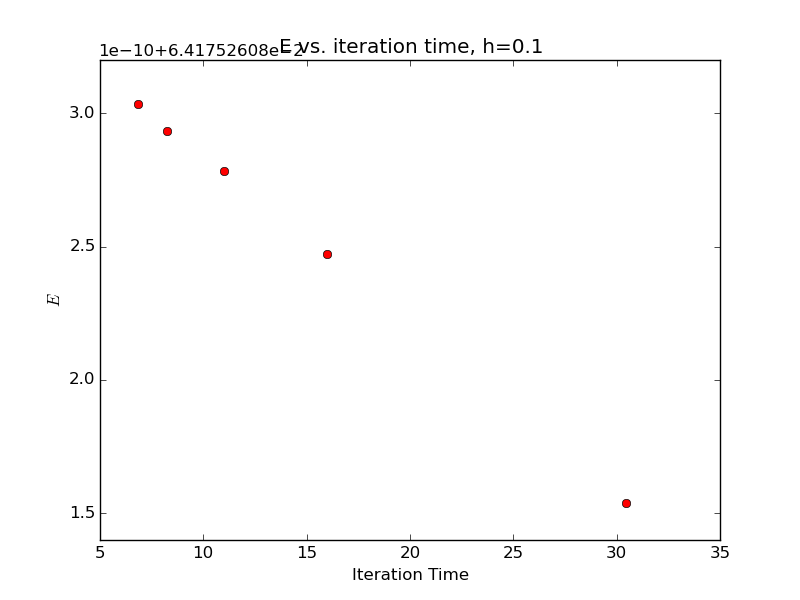
\includegraphics[width=.6\textwidth]{homework7_problem1_plot24}
\end{figure}
\begin{figure}[H]
  \centering
    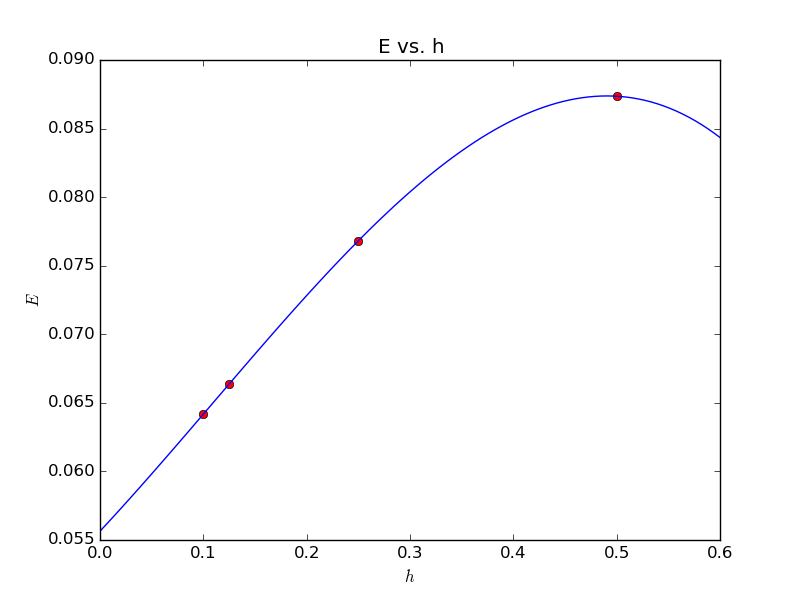
\includegraphics[width=.6\textwidth]{homework7_problem1_plot25}
\end{figure}

\subsection{Analysis and Interpretation}

It is very clear from the plots above that the solution becomes much better with smaller choices in lattice spacing $h$. The ``energy'' $E$ also does not change with choice of $w$, which is expected.

The case where $E(h\rightarrow0)$ is also extrapolated using a third degree polynomial fit (using numpy's built in solver). This value appears to be fairly consistent with what we would expect as we get finer mesh spacings. With this extrapolated data, we would expect that $E(h=0) = 0.0526225166753.$

It is fairly aparent that this is actually an underestimation, as the analytic results yields that $E=0.0611965006177$ when $h=0.1$, and as the step size is scaled downward the solution tends to go toward $E=0.058$.

Plots showing the iteration times for different $E$ values given a static lattice spacing $h$ and changing $w$ are also shown, as requested. These are primarily to demonstrate that the value does not change with choice of $w$, but the solution time does change significantly. While they do not appear to be the same by the plot, if one notes that scale of the y-axis we see that the difference between the points are well below machine precision.

Finally, the solutions themselves are obviously better with smaller spacing. The worst case, where there are only 3 points in the $x$ domain, is more or less garbage. As the spacing gets better we see a better solution, which is reminiscent of heat dissipation, which can be described by Laplace's equation.

\subsection{Log}

This program took approximately 14 hours.

\pagebreak

\section{Problem 2}

\subsection{Problem Statement}


Write a code to solve the following diffusion equation using (i) the explicit scheme (10 pts), (ii) the
implicit scheme (15 pts), and (iii) more sophisticated scheme (15 pts):

$$ \frac{\partial \phi}{\partial t} = \frac{\partial^2 \phi}{\partial x^2}$$

with

$$\phi(0,t) = \phi(2, t) = 0,$$
$$\phi(x,t=0) = x \text{ for } 0 \le x \le 1, -x+2 \text{ for } 1\le x \le 2$$

The explicit scheme is implemented as

$$\phi^{n+1} = (1-H\Delta t)\phi^n $$

The implicit scheme is implemented as

$$\phi^{n+1} =\frac{1}{1+H\Delta t} \phi^n$$

More sophisticated scheme is implemented as

$$\phi^{n+1} =\frac{1-\frac{1}{2}H\Delta t}{1+\frac{1}{2}H\Delta t} \phi^n$$

where the superscript denotes the time step, $H(\phi_i) = -(\phi_{i+1} + \phi_{i-1} - 2\phi_i)/h^2$
, and $h$ is a lattice spacing.

You may use the number of lattice points $N$ as 50 and use two different time steps such as $\Delta t=0.00075$
and $\Delta t=0.001$. Find the solution $\phi(x, t)$ for $t=0.005, 0.01, 0.02, 0.03,$ and $0.045$.

(i) When each scheme is implemented, check if your numerical solution is stable with $\Delta t=0.0007$
and $\Delta t=0.001$, as time evolves. Show this in the two figures. One figure is for $\Delta t=0.0007$, and
the other figure is for $\Delta t=0.001$. In each figure, $\phi(x, t)$ as a function of x and t can be plotted.
For example, $\phi(x, t)$ vs $x$ for each $t$ value can be included in each figure (five curves in one
figure).

(ii) When the implicit scheme is used, compare the numerical solution $\phi(x, t)$ with the analytical
solution. Show this in a figure by plotting a difference between between the numerical and
analytical solutions, as a function of $x$ and $t$ for the two different $\Delta t$ values.

(iii) When the sophisticated scheme is used, compare this numerical solution $\phi(x, t)$ with the
solution you obtained from (ii). Compare this solution with the analytical solution. Show this
in figures.

(iv) Which one among the three schemes is the most accurate?

\subsection{Method}

The method in this problem is fairly straightforward. Each of the schemes are implemented as described in the problem statement, each run with different time steps and plotted as described in the problem statement.

\subsection{Verification of Program}

This program was verified by comparing it to the analytical solution, which is shown later.

\pagebreak

\subsection{Data}
The results of the problem are shown in the plots below.
\begin{figure}[H]
  \centering
    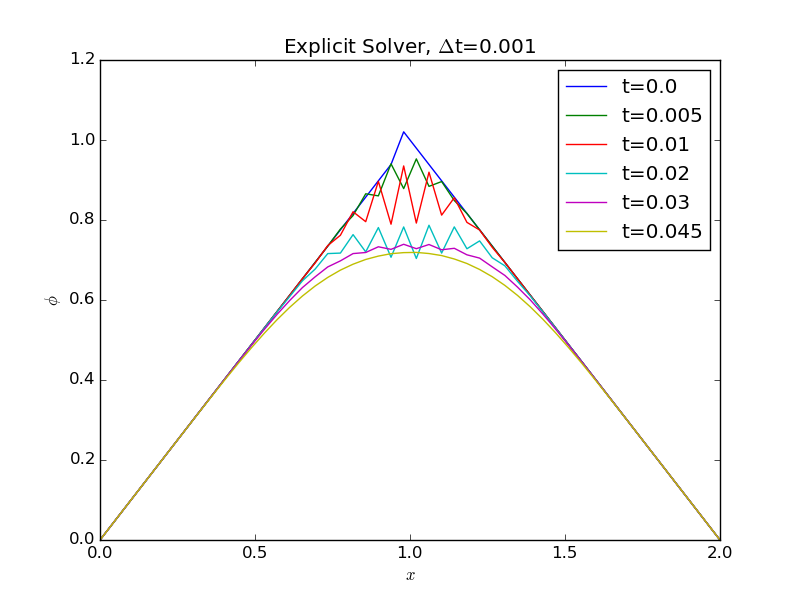
\includegraphics[width=.6\textwidth]{homework7_problem2_plot0}
\end{figure}
\begin{figure}[H]
  \centering
    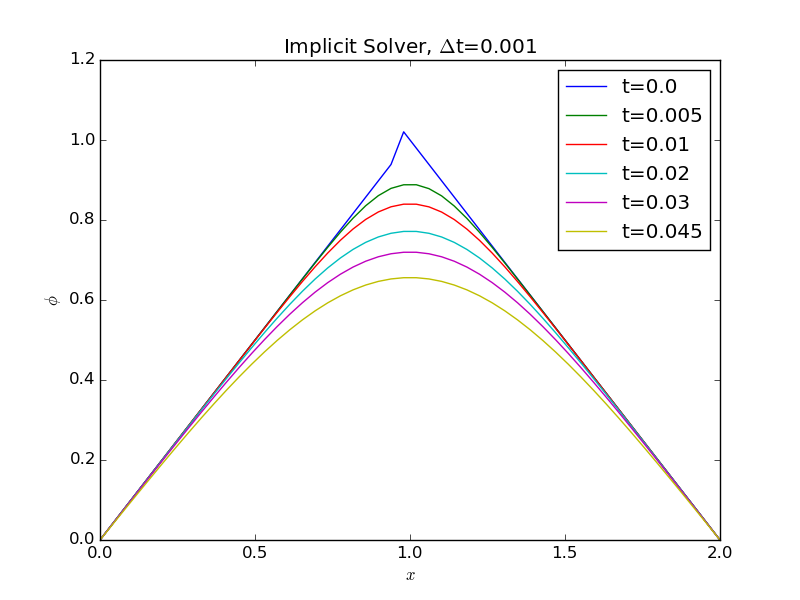
\includegraphics[width=.6\textwidth]{homework7_problem2_plot1}
\end{figure}
\begin{figure}[H]
  \centering
    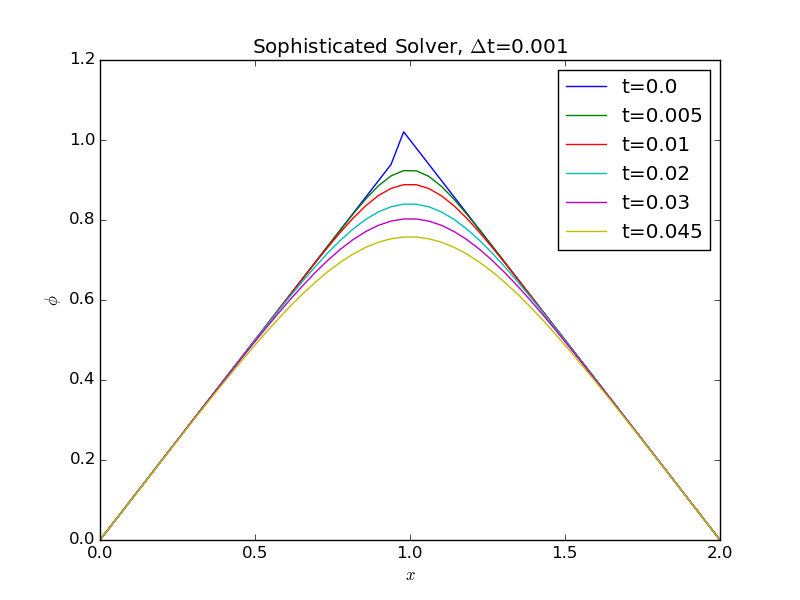
\includegraphics[width=.6\textwidth]{homework7_problem2_plot2}
\end{figure}
\begin{figure}[H]
  \centering
    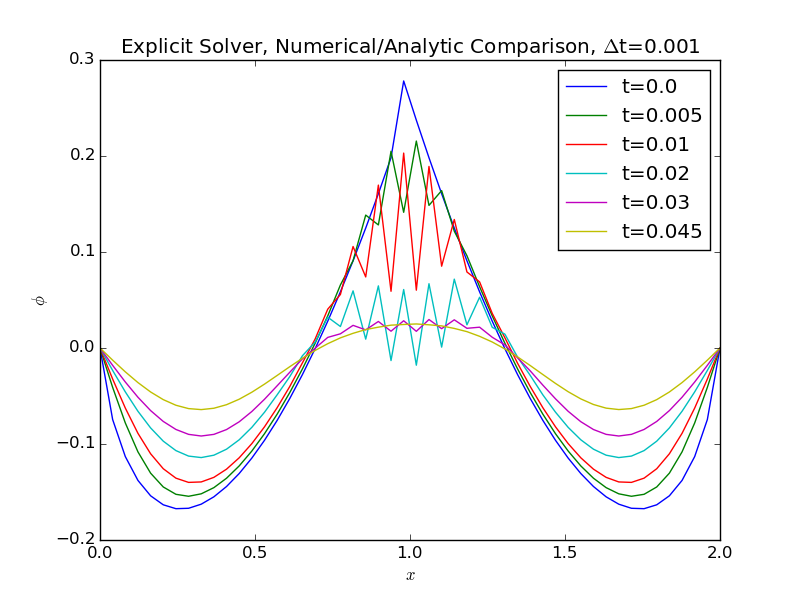
\includegraphics[width=.6\textwidth]{homework7_problem2_plot3}
\end{figure}
\begin{figure}[H]
  \centering
    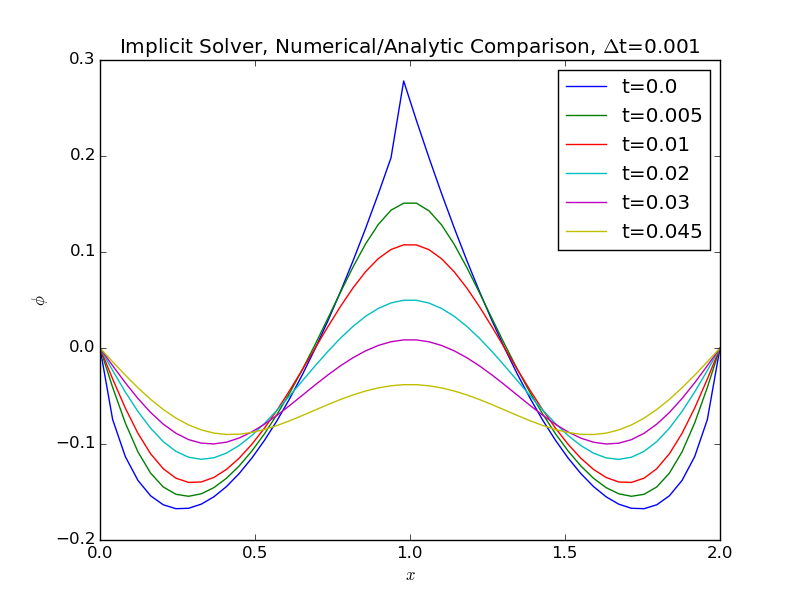
\includegraphics[width=.6\textwidth]{homework7_problem2_plot4}
\end{figure}
\begin{figure}[H]
  \centering
    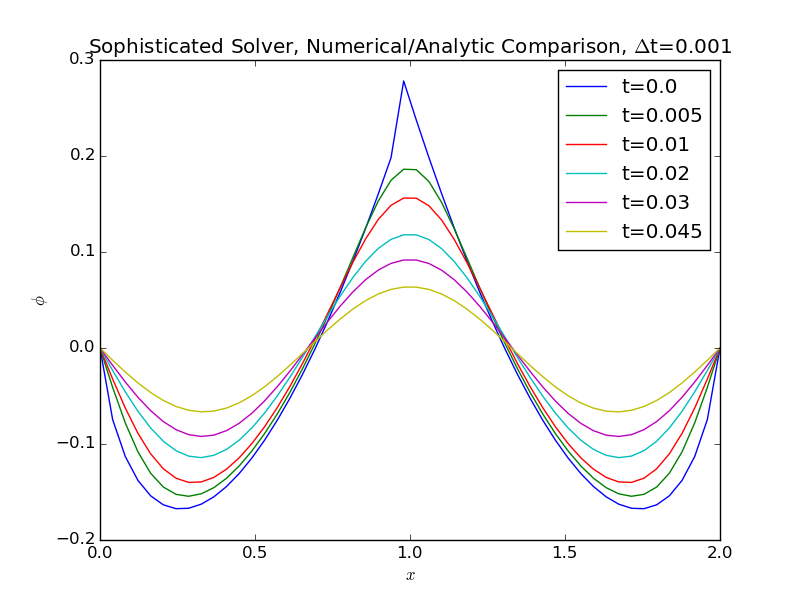
\includegraphics[width=.6\textwidth]{homework7_problem2_plot5}
\end{figure}
\begin{figure}[H]
  \centering
    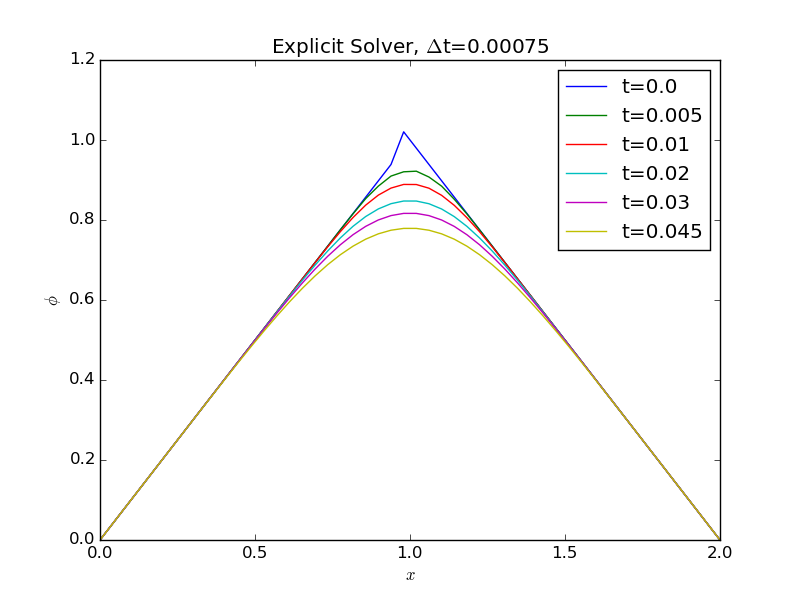
\includegraphics[width=.6\textwidth]{homework7_problem2_plot6}
\end{figure}
\begin{figure}[H]
  \centering
    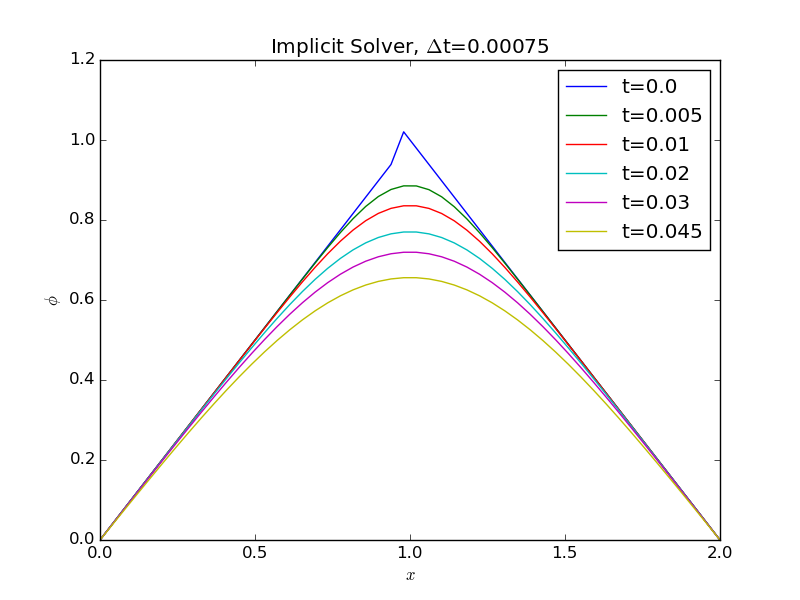
\includegraphics[width=.6\textwidth]{homework7_problem2_plot7}
\end{figure}
\begin{figure}[H]
  \centering
    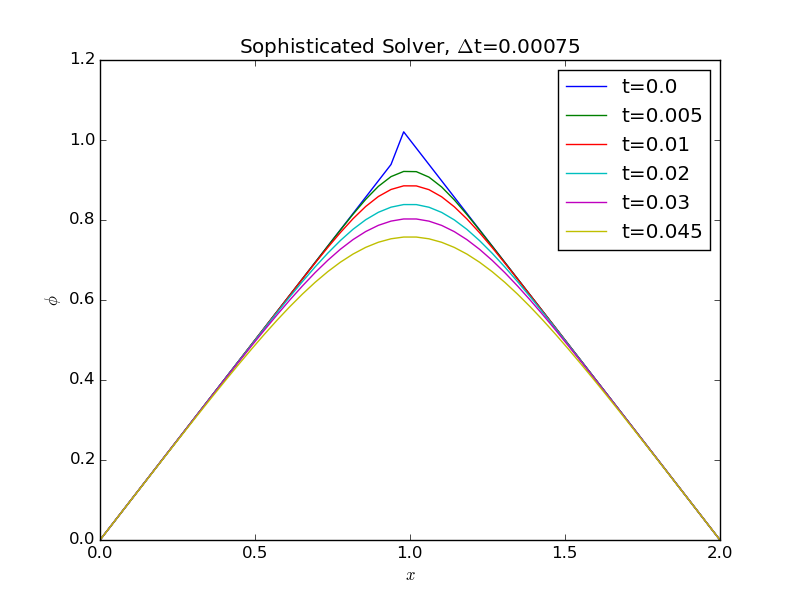
\includegraphics[width=.6\textwidth]{homework7_problem2_plot8}
\end{figure}
\begin{figure}[H]
  \centering
    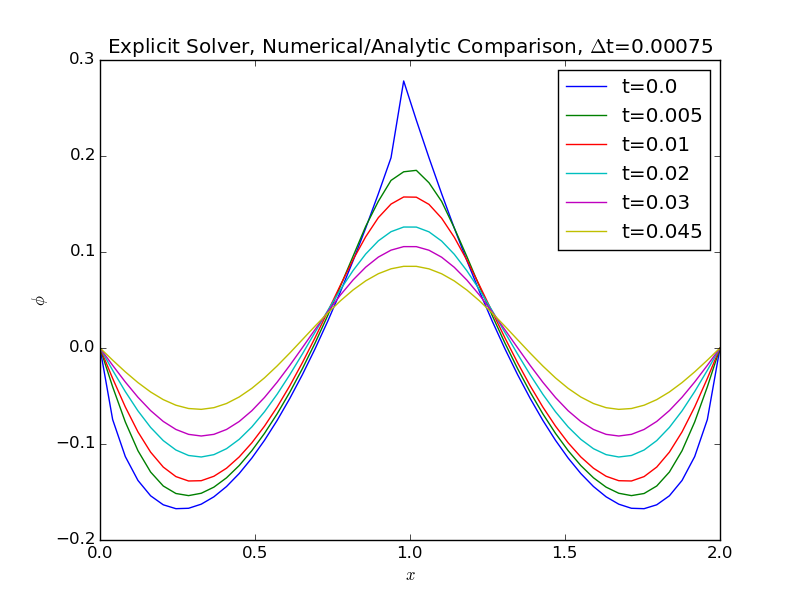
\includegraphics[width=.6\textwidth]{homework7_problem2_plot9}
\end{figure}
\begin{figure}[H]
  \centering
    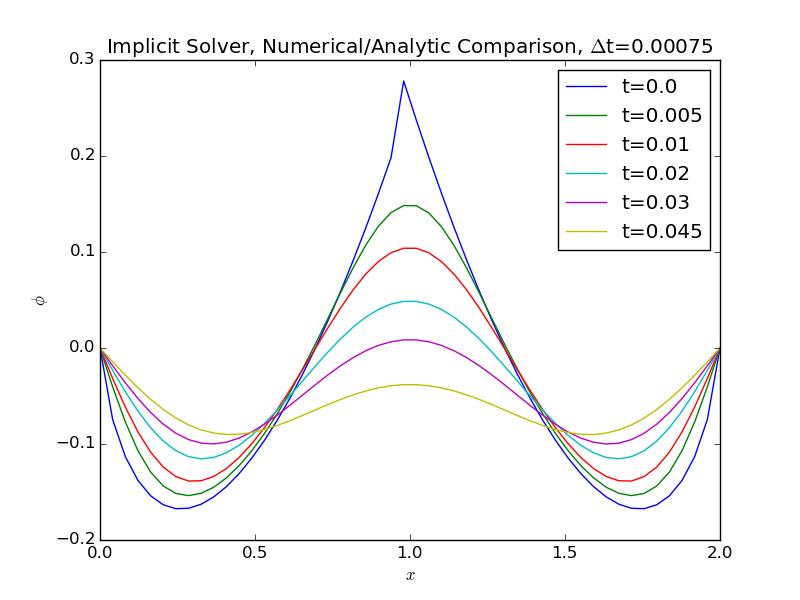
\includegraphics[width=.6\textwidth]{homework7_problem2_plot10}
\end{figure}
\begin{figure}[H]
  \centering
    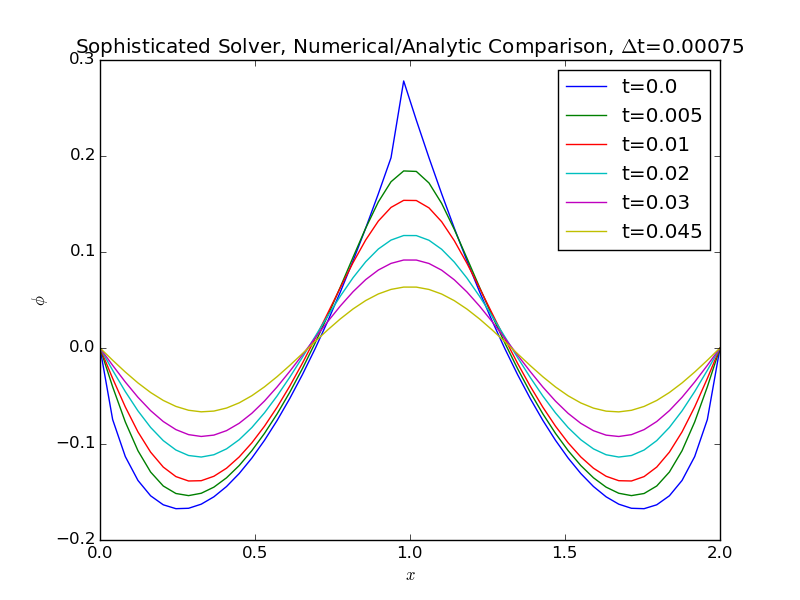
\includegraphics[width=.6\textwidth]{homework7_problem2_plot11}
\end{figure}

\pagebreak
\pagebreak
\subsection{Analysis}

It is apparent that the numerical solutions are not stable for $\Delta t = 0.001$, as seen by the plots comparing the numerical and analytic values. The analytic solution was taken from the lecture notes, and given as

$$\phi(x,t) = 8\sum_{n=0}^{\infty} \frac{(-1)^n}{(2n+1)^2\pi^2}\exp{\left[-\frac{(2n+1)^2\pi^2t}{4}\right]}\sin{((n+\frac{1}{2})\pi x)} .$$

\begin{figure}[H]
  \centering
    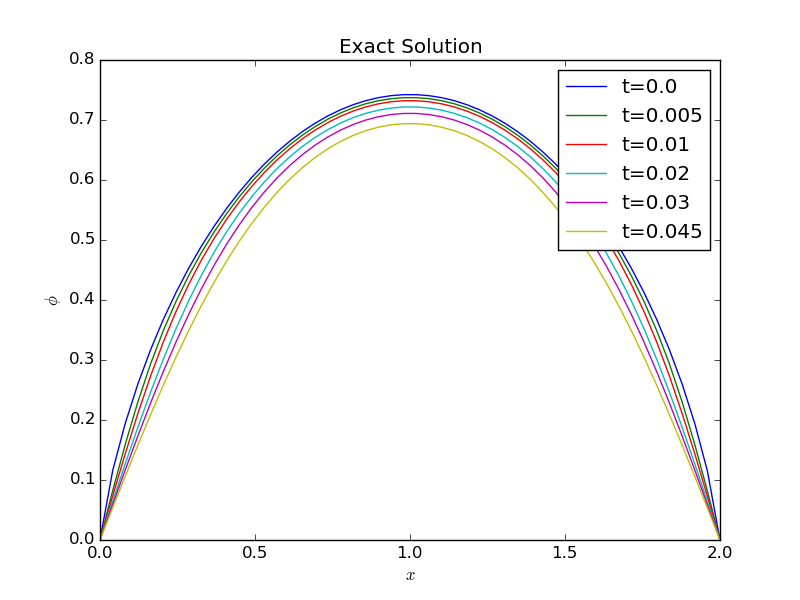
\includegraphics[width=.6\textwidth]{homework7_problem2_plot-1}
\end{figure}

It is very clear that the less-refined time step is unstable near the top of our solution, where jagged solution values begin to appear. This is especially significant in the explicit solver. This issue is not shown in the finer time step choice, which is to be expected.

The solution also do not appear to completely converge to the intended solution, as we expect. Instead, the solution is somewhat sinusoidal in nature. It does appear, however, that allowing the solution to progress to further time steaps would solve this issue, and the solution would converge to the expected one.

Further, it appears that the implicit solver actually handles the solution with a significant underestimation, and after a significant time evolution would not converge to the expected solution. Regardless, but the implicit and sophisticated solvers are much better than the explicit solver. In the case of the sophisticated solver, it even appears that the numerical solution would converge to the analytic solution within a fairly small time frame.

\subsection{Interpretation}

This problem, while it had issues comparing to the analytic value, does appear to show the intended results; the stability of the solution is very heavily dependent on the choice of $\Delta t$.
 
\subsection{Log}

This problem took about 5 hours to complete.

\end{document}